%============================================================================
\section{Testing and Optimizing the Algorithm}\label{chap:tests}
%============================================================================

The current implementation of our merger tree algorithm needs several
free parameters to be chosen by the user. We present in this section
multiple tests that reveal the recommended values for these
parameters.  We use for this a single reference cosmological
simulation and analyze the merger trees we obtained for different set
of parameters.  A similar methodology was used in the Sussing Merger
Trees Comparison Project \citep{SUSSING_COMPARISON,
  SUSSING_CONVERGENCE, SUSSING_HALOFINDER,leeSussingMergerTrees2014a}.
This is why we adopt in this section several tests from this seminal
work, as they are quite efficient at testing the strengths and the
weaknesses of merger tree codes. They also allow for a direct
comparison of our new implementation with many other state-of-the-art
merger tree codes in the community.

%============================================================================
\subsection{Test Suite}\label{chap:testing_methods}
%============================================================================

We now list the different diagnostics we use to characterize the quality of
our merger tree algorithm.

\begin{enumerate}
  \setlength\itemsep{1em}
\item \emph{Length of the Main Branch of a Halo}
  
  The length of the main branch of a halo is simply defined as the
  number of snapshots in which a halo and all its progenitors are
  detected.  A halo at $z=0$ without any progenitors will be
  considered as newly formed and thus will have a main branch of
  length $1$.  If a halo appears to merge temporarily into another and
  re-emerges at a later snapshot, the missing snapshots will be
  counted towards the length of the main branch as if they weren't
  missing. Traditionally, finding long main branches is considered
  as a good thing for a merger tree code.
  
\item \emph{Number of Branches of a Halo}
  
  Another popular quantity is the number of branches of the tree
  leading to the formation of a halo at $z=0$.  The main branch is
  included in this count, thus the minimal number of branches is
  $1$. If a different choice of parameters leads to a reduction of the
  number of branches, it usually corresponds to an increase of the
  average length of the main branches and a smaller number of merger
  events. For example, intuitively if we compare the merger trees where
  we use only one tracer particle per clump to the trees that were built 
  using several hundreds tracer particles per clump, we would expect to 
  be able to detect more fragmentation events with the increased number of 
  tracer particles. If the fragmentation remained undetected, we would 
  instead have found a newly formed clump (the fragment) alongside a 
  merging event. Both the ``newly formed'' fragment as well as its
  progenitor, which is now merged into a descendant, will have shorter
  main branches. Conversely, the descendant will have an increased 
  number of branches compared to the scenario where the fragmentation
  was detected.
  Finally, in the hierarchical picture of structure formation, one
  would expect more massive clumps to have longer main branches and a
  higher number of branches.
  
\item \emph{Logarithmic Mass Growth of a Halo}
  
  The logarithmic mass growth rate of a halo is computed using the following
  finite difference approximation:
  %
  \begin{equation}
    \frac{\de \log M}{\de \log t} \simeq
    \frac{(t_{k+1}+t_{k})(M_{k+1} -M_{k})}{(t_{k+1} - t_k)(M_{k+1} +
      M_{k})} \equiv \alpha_M(k, k+1)
  \end{equation}
  %
  where $k$ and $k+1$ are two consecutive snapshots, with the
  corresponding halo mass $M_k$ and $M_{k+1}$ and times $t_k$ and
  $t_{k+1}$. A convenient approach was proposed by \cite{SUSSING_CONVERGENCE}
  to reduce the range of values to the interval $(-1, 1)$ using the new variable
  %
  \begin{equation}
    \beta_M = \frac{2}{\pi}\arctan(\alpha_M) \label{eq:massgrowth}
  \end{equation}
  %
  Note that we expect the mass of dark matter haloes to increase
  systematically with time.  We also expect in some cases the mass to
  remain constant or even to decrease slightly.  We nevertheless
  expect the distribution of $\beta_M$ to be skewed towards $\beta_M >
  0$.  $\beta_M \rightarrow \pm 1$ imply $\alpha_M \rightarrow \pm
  \infty$, indicating suspiciously extreme cases of mass growth or
  mass loss.
  
\item \emph{Mass Growth Fluctuation of a Halo}
  
  Mass growth fluctuations are defined similarly as
  %
  \begin{equation}
    \xi_M = \frac{\beta_M(k, k+1) - \beta_M(k-1, k)}{2} \label{eq:massfluct}
  \end{equation}
  %
  where $k-1$, $k$, $k+1$ are three consecutive snapshots.  A smooth
  mass accretion history generally leads to $\xi_M \simeq 0$.  Strong
  deviations from zero could indicate an erratic behaviour, indicating
  extreme mass loss followed by extreme mass growth and vice versa.
  Within the standard model of structure formation, this behaviour is
  expected only during major merger events. Otherwise, it might
  indicate either a misidentification by the merger tree code or a
  misdetection by the halo finder.

%\item {\it Displacement statistics}
%  The Sussing Merger Trees Comparison Project also includes a
%  displacement statistic to quantify misidentifications,
%  \begin{equation}
%  \Delta_r = \frac { | \mathbf{r}_{k+1} - \mathbf{r}_k - 0.5
%    (\mathbf{v}_{k+1} + \mathbf{v}_k) (t_{k+1} - t_k) | } {
%    0.5(R_{200,k} + R_{200,{k+1}} + | \mathbf{v}_{k+1} + \mathbf{v}_k
%    | (t_{k+1} - t_k) }
%  \end{equation} 
%  where $\mathbf{r}_{k+1}$, $\mathbf{v}_{k+1}$ and $\mathbf{r}_k$,
%  $\mathbf{v}_k$ are the position and velocity of a clump at snapshot
%  $k+1$ and its progenitor at snapshot $k$, respectively; $t_{k+1}$
%  and $t_k$ are the cosmic times at which the two clumps were defined,
%  and $R_{200}$ is the radius that encloses an overdensity of 200
%  times the critical density $\rho_{c} = \frac{3 H^2}{8 \pi G}$.
%  Values of $\Delta_r > 1$ would indicate a misidentification, so the
%  parameters minimising $\Delta_r$ should be preferred, provided the
%  acceleration is approximately uniform.  However, the obtained
%  $\Delta_r$ for all parameters showed almost no differences and no
%  indication of what parameters should be preferred, which is why the
%  results of the quantification of misidentifications were omitted
%  from this work.
 
\end{enumerate}

Ideally, we should have tested \texttt{ACACIA} on the dataset used in
\citet{SUSSING_COMPARISON} and \citet{SUSSING_HALOFINDER} (S13 and A14
from here on, respectively).  This would
have enabled a direct comparison of the performance to other merger
tree codes.  However, \texttt{ACACIA} was designed to work on the fly
with the \ramses\ code.  Using it as a post-processing tool would
defeat its purpose and as a matter of fact handling other halo 
catalogues  has proven technically impossible. \texttt{ACACIA} is 
tightly coupled to the \phew\ halo finder, and relies heavily on 
already existing internal structures and tools, in particular the 
explicit communications which are necessary for parallelism on 
distributed memory architectures, as well as the structures and 
their hierarchies as they are defined by \phew. Attempting to use 
other halo catalogues would require us to re-write a significant 
portion of the \phew\ halo finder. If we instead used only particle
data, which is possible, we would still find a different halo catalogue
compared to other structure finding codes, and we would still not be
able to do an exact comparison. Furthermore, we also want to demonstrate that the
\phew\ halo finder can be used within the \ramses\ code to produce
reliable merger trees.  For these various reasons, we have decided to
perform the same tests but using our own dataset generated on the fly by
\ramses.

Despite this limitation, we have performed a direct comparison to
other halo finders and merger tree codes using the exact same merger
tree parameters as in A14. The results are
given in Appendix~\ref{app:performance_comparison}.  Our results are
comparable to e.g. the \texttt{MergerTree}, \texttt{TreeMaker} and 
\texttt{VELOCIraptor} tree builders with \texttt{AHF}, \texttt{Subfind},
or \texttt{Rockstar} halo finders as presented in A14, demonstrating that
\texttt{ACACIA} performs similarly than other state-of-the-art tools.


In this section, we would like to explore different parameters and see
how they affect the quality of the merger tree.  Our tests are
performed on a single DMO simulation with $256^3 \approx 1.7\times
10^7$ particles of identical mass $m_p = 1.6\times 10^9\msol$. To enable
a comparison with A14, we adapted the same cosmology
and snapshot output times as them at a comparable, but slightly lower
resolution. The cosmological parameters used are taken from the WMAP-7 
\citep{komatsuSevenYearWilkinsonMicrowave2011}, while the snapshot times 
are identical to the ones used for Millenium Simulation 
\citep{springelSimulationsFormationEvolution2005a}, starting at redshift
50 and being roughly uniformly spaced in log $a$ in 61 steps. 
At redshift zero, the simulation was then continued for 3 further snapshots 
to ensure that the merging events at $z = 0$ are actual mergers and not 
temporary mergers that will re-emerge later.

This choice of spacings between the snapshots was relatively
arbitrarily in the sense that we did not take into account any further
underlying physical considerations that would be important in e.g.
semi-analytical models. For different snapshot spacings, we recommend to 
follow the suggestions found by \citet{SUSSING_CONVERGENCE}:

\begin{itemize}
\item  Sequences of snapshots with very rapidly changing time intervals 
between them should be avoided as they can lead to very poor trees.
\item  Increasing the number of outputs from which the tree is generated 
results in shorter trees. This is because, due to limitations in the input halo 
catalogue, tree-builders may face difficulties caused by the fluctuating center 
and size of the input haloes, and the frequency of detected temporary merging 
events increases with the number of snapshots, resulting in haloes missing from
the catalogue. For merger trees built from
an order of 100 or more snapshots, they recommend using an algorithm capable of
dealing with these problems, which \texttt{ACACIA} is able to do, although at the
moment this patching of missing haloes in the catalogue isn't based on a physical
timescale, but on a user defined number of snapshots.
\item  To facilitate this patching at the end of the simulation, snapshots should 
be generated beyond the desired endpoint. This would entail typically running past 
$z = 0$, as we did with our test suite. 
\end{itemize}

For the clump finder, we have adopted a outer density
threshold of 80$\bar\rho$ and a saddle surface density threshold of
200$\bar\rho$, where $\bar\rho = \Omega_m \frac{3 H^2}{8 \pi G}$ is
the average density.  The minimal mass for clumps is set to 10
particles. Note that for the histogram of the logarithmic mass growth
and mass growth fluctuations, we adopt a threshold for the clump mass
of 200 particles for sake of visibility. Choosing a smaller mass
threshold would indeed give too much weight to small mass, poorly
resolved haloes in our statistical analysis.




%==========================================================================================
\subsection{Varying the Clump Mass Definition}\label{chap:varying_clump_mass_definition}
%==========================================================================================

In our current implementation, there are two important parameters that
can have a strong effect on the halo catalogue (beside the mass and
the density thresholds mentioned earlier) and the corresponding merger
tree.

The first one is the exact definition adopted for the mass of the
sub-haloes in the merit function.  For main haloes, there is no
ambiguity as the mass is defined as the sum of the masses of all
particles contained within the boundary of the halo (set by the outer
density isosurface). This is not the case for sub-haloes, because of the
unbinding process described in Section~\ref{chap:phew}. Indeed,
unbound particles are removed from their original sub-halo and passed
to the parent sub-halo in the hierarchy.  Clump masses are therefore
defined as the sum of the mass of all bound particles.  In the merit
function evaluation, we however consider two different cases to
compute the mass: 1- the mass is equal to the sum of the masses of
only the bound particles, like for sub-haloes or 2- the mass is equal
to the sum of the masses of all particles within their boundaries (set
by the saddle surface with neighbouring clumps), like for main haloes.
In the former case, the mass used in the merit function is identical
to the clump mass. It is referred to as the \exc\ case.  In the latter
case, the mass in the merit function is different that the sub-halo
mass definition but identical to the main halo mass definition.  We
refer to this case as \inc.

The second important definition is the exact boundedness criterion
adopted for the unbinding process.  As discussed in
Section~\ref{chap:phew}, we explored two different cases: When
particles are allowed to leave the outer boundary of their host clump
(and possibly come back later) or when particles are not allowed to
cross the saddle surface during their orbital evolution. In the first
case, we only require the binding energy to be negative, while in the
second case, the binding energy has to be smaller than the
gravitational potential of the nearest saddle point.  We call the
first case \nosad\ and the second case \sad.

\begin{figure*}
  \centering
  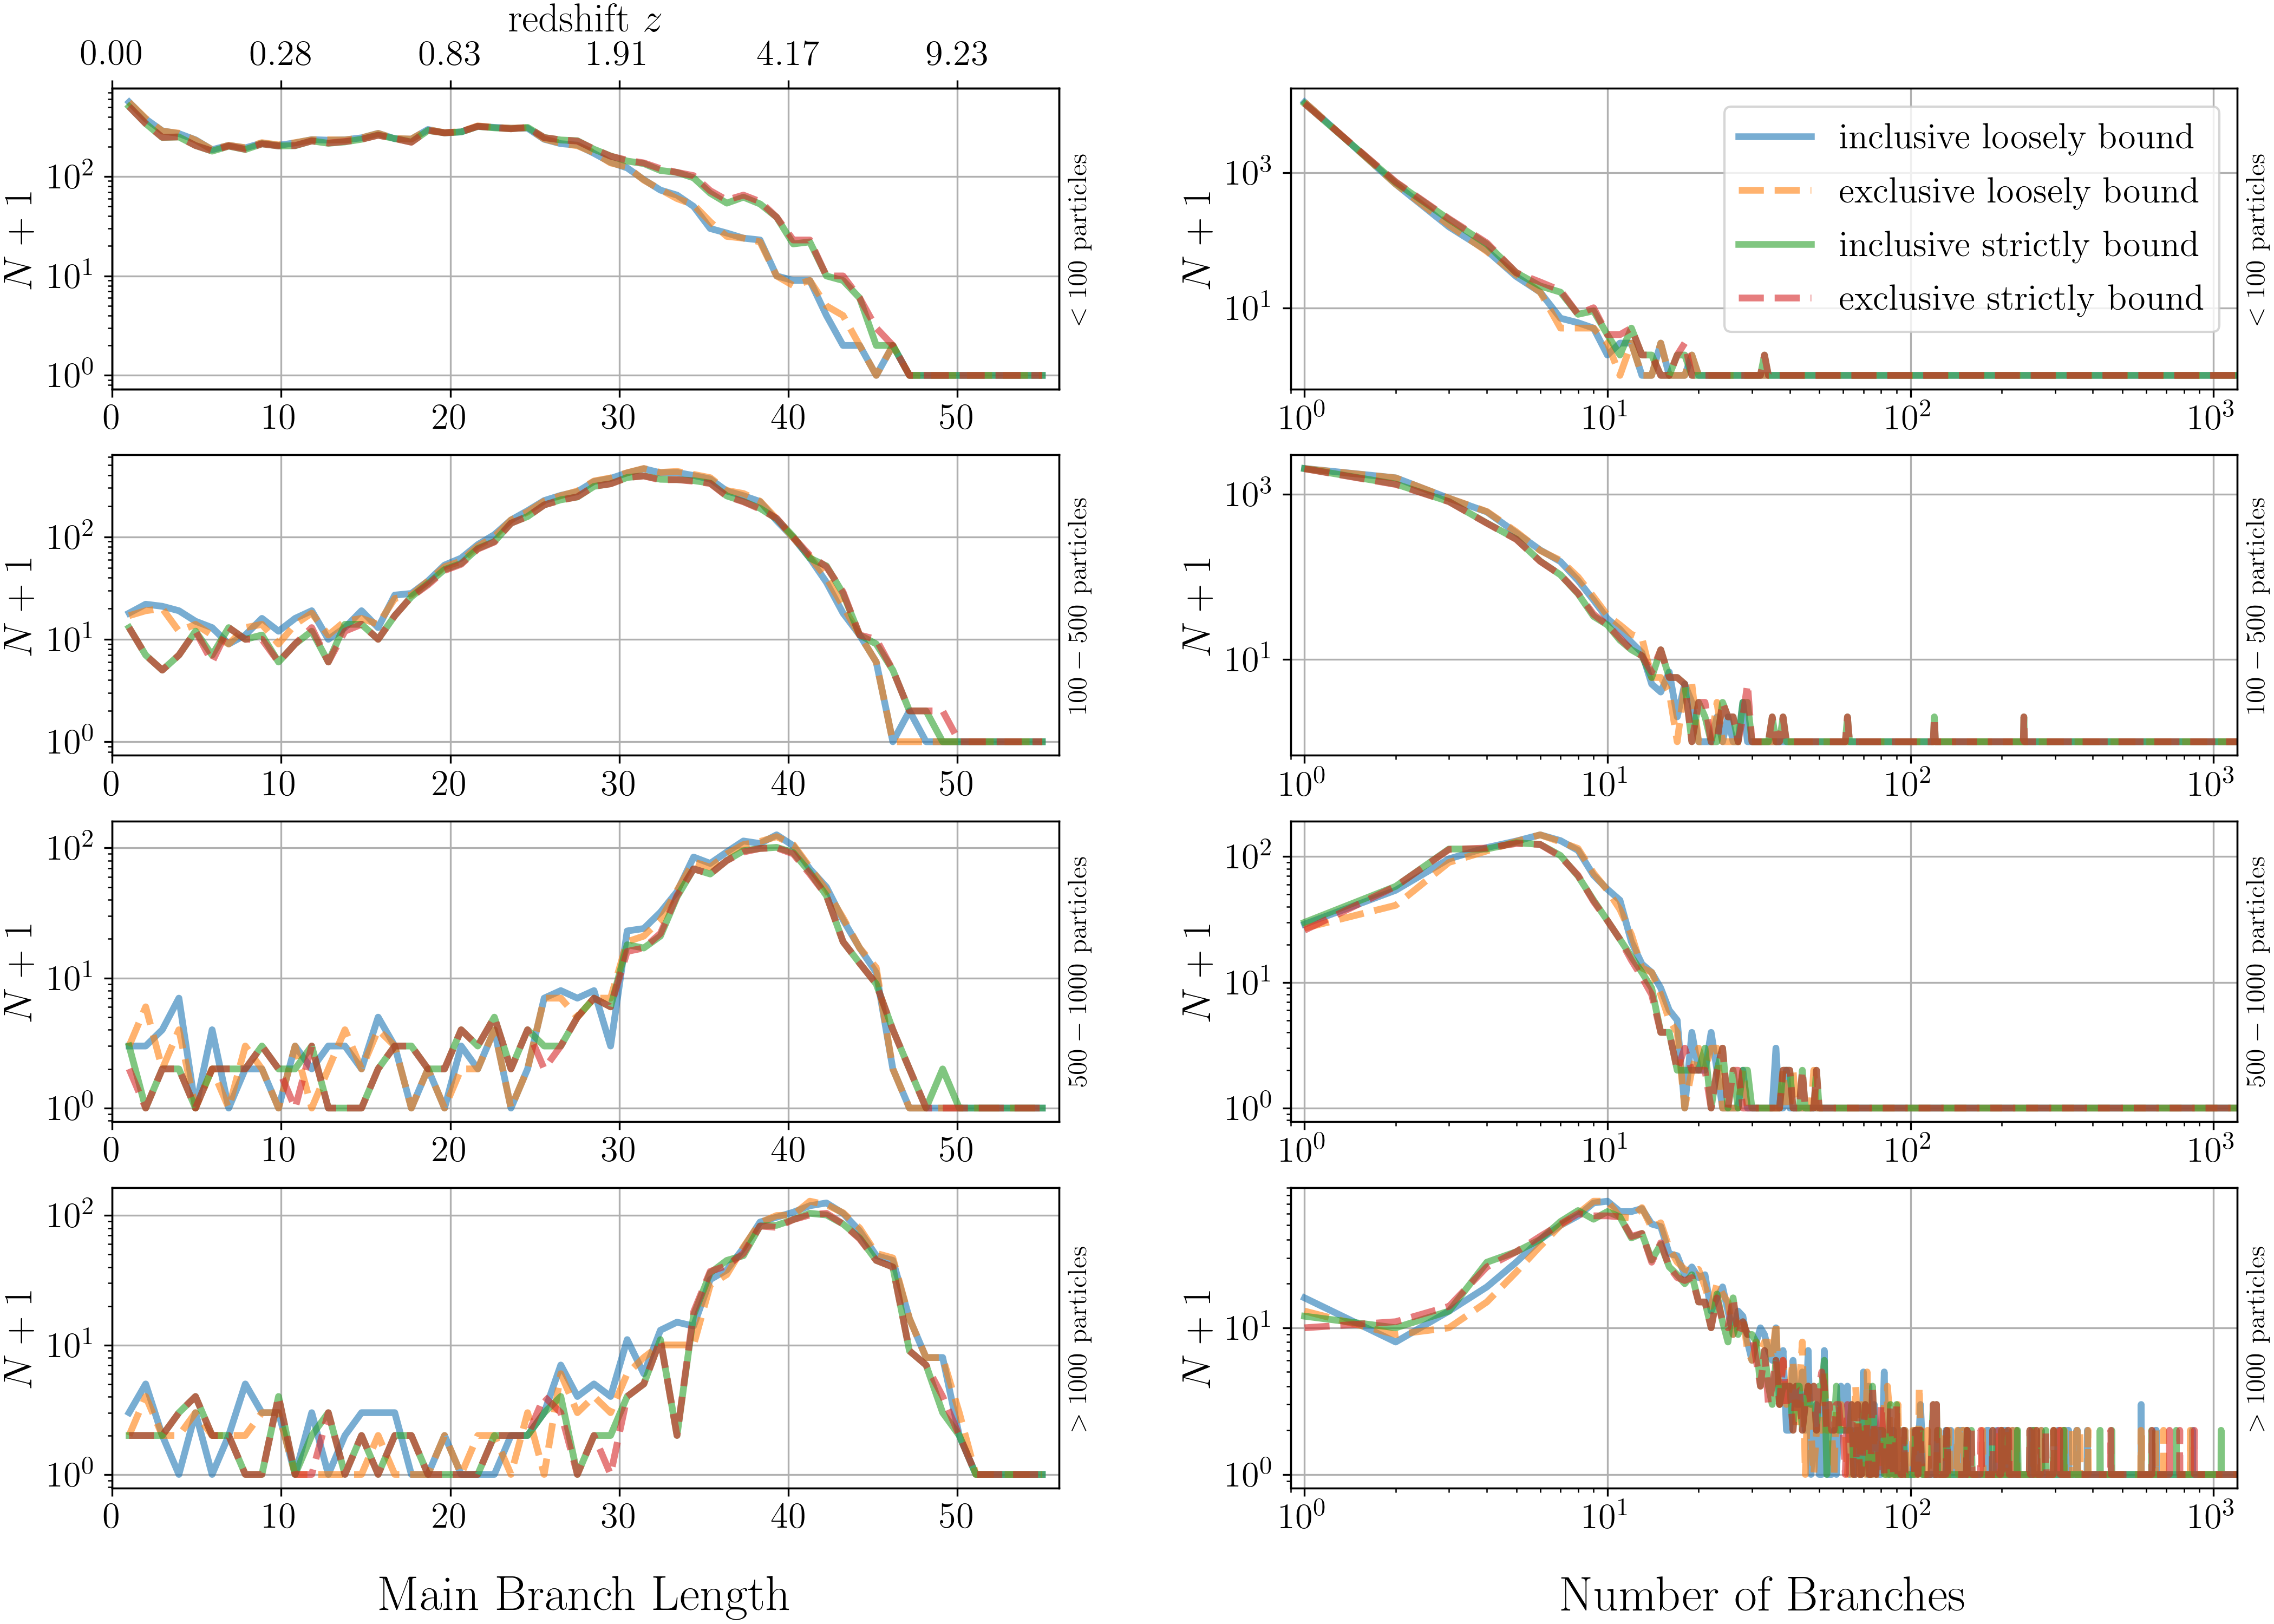
\includegraphics[width=\textwidth,keepaspectratio]{images/tree-statistics-my-threshold/tree_geometry-inc-excl.png}
  \caption{Histogram of the length of main branch (left) and of the
    number of branches (right) for all clumps (halo and sub-halo)
    detected at $z=0$. Each row corresponds to a different range of
    clump masses (expressed in particle numbers): less then 100 (top),
    100-500, 500-1000 and more than 1000 (bottom). We compare these
    histograms for four different cases: whether unbound particles are
    included (\inc) or excluded (\exc) in the evaluation of the merit
    function, and whether bound particles are \nosad\ or \sad.
  }%
  \label{fig:saddle_nosaddle_mbl_nbranch}
\end{figure*}

\begin{figure}
  \centering
  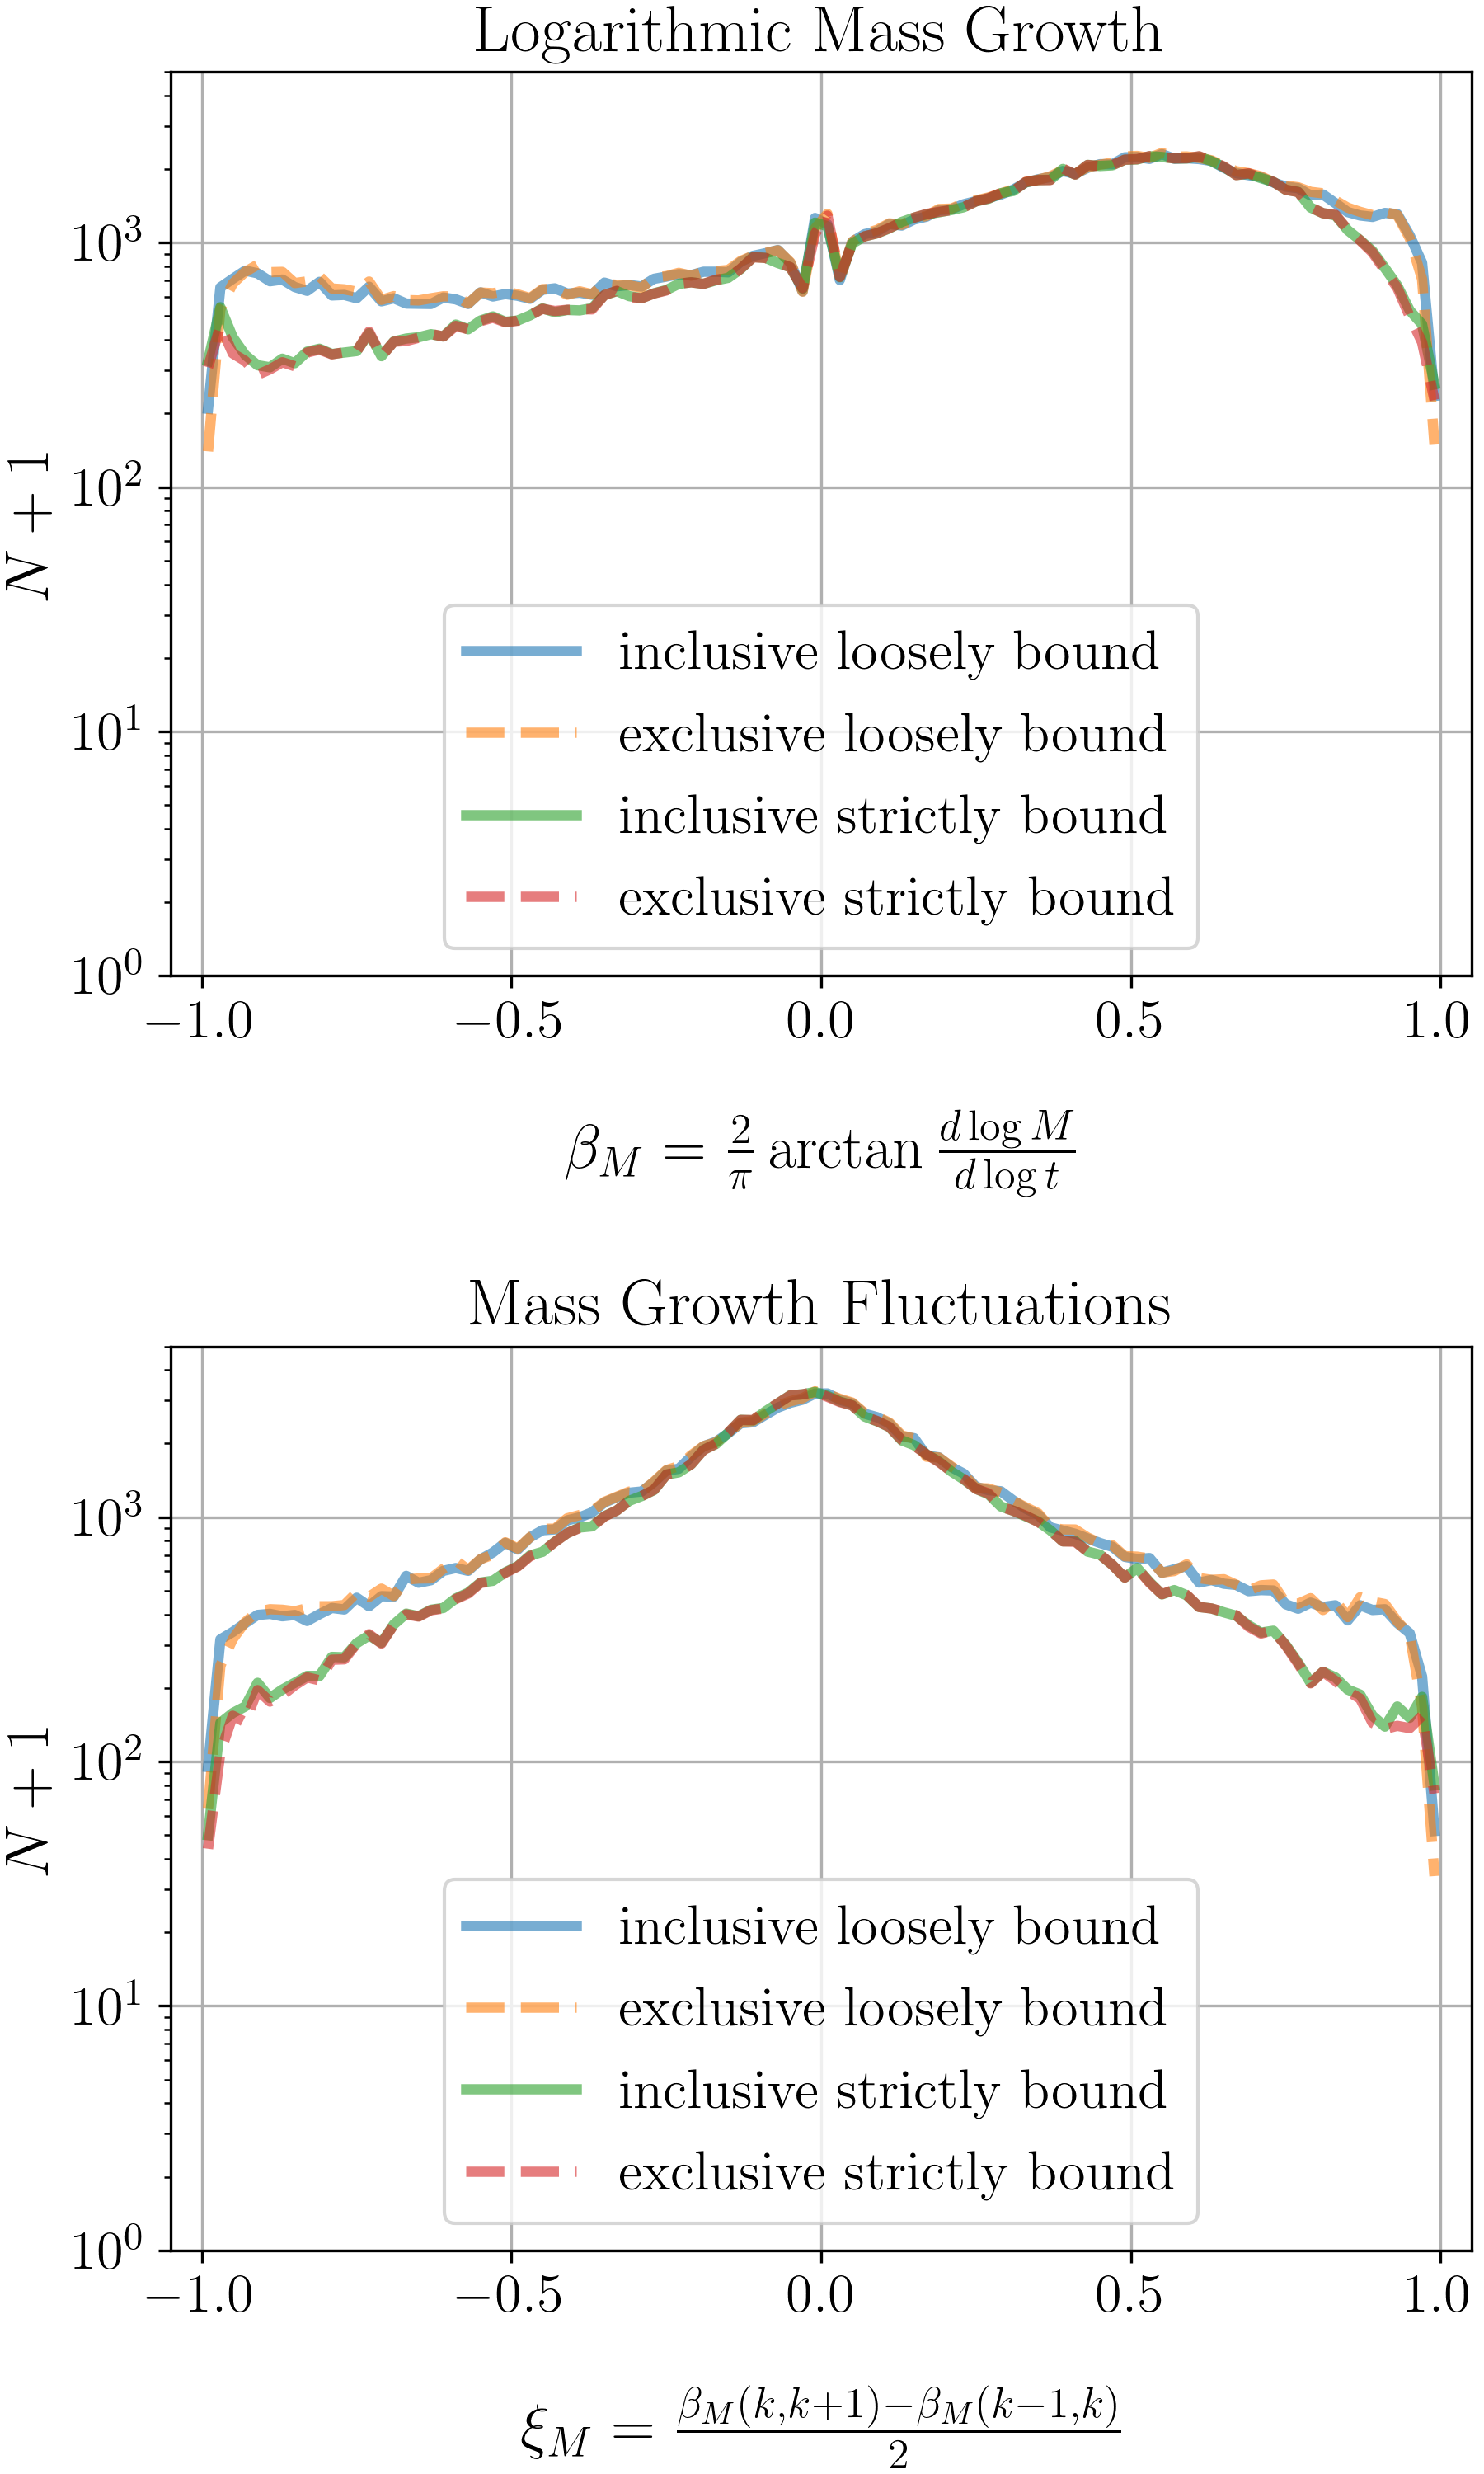
\includegraphics[width=.9\linewidth, keepaspectratio]{images/tree-statistics-my-threshold/mass-statistics-inc-excl.png}%
  \caption{Histogram of the logarithmic mass growth (top) and the mass
    growth fluctuation (bottom) for all clumps (halo and sub-halo)
    detected in two (top) or three (bottom) consecutive snapshots of
    the simulation and with more than 200 particles. We compare these
    histograms for four different cases: whether unbound particles are
    included (\inc) or excluded (\exc) in the evaluation of the merit
    function, and whether bound particles are \nosad\ or \sad.
  }%
  \label{fig:saddle_nosaddle_masses}
\end{figure}

\begin{table*}
	\caption{
        Average data for all clumps at $z=0$ depending on whether to consider particles which might wander off into another clump as bound (\nosad) or not (\sad).
        The results shown are for the \exc\ mass definition, which show no significant difference to when the \inc\ mass definition is used.
%        The groups I, II, III and IV are defined as clumps that contain less then 100, 100-500, 500-1000 or more than 1000 particles, respectively.
        \label{tab:saddle_nosaddle}
    }
        
%	{\small 
%		\begin{tabular}[c]{l | p{2.8cm} | p{2.8cm} |}
%													&	 \sad\  &   \nosad\ \\ 
%			
%			\hline
%			%
%			total clumps	 						&	 16262	& 	17242 	\\			
%			%		
%%			max number of particles in a clump 		&	 414570	& 	271438 	\\			
%			%		
%			median number of particles in a clump 	&	 83		& 	93 		\\			
%			%
%			\hline
%			%		
%			average main branch length group I		&	23.153	& 	20.527 	\\			
%			%
%			average main branch length group II		&	48.835	& 	48.642 	\\			
%			%		
%			average main branch length group III	&	54.715	& 	54.904 	\\			
%			%
%			average main branch length group IV		&	53.958	& 	56.265 	\\			
%			%
%			\hline
%			%		
%			average number of branches group I		&	1.327	& 	1.230 	\\			
%			%
%			average number of branches group II		&	3.448	& 	3.603 	\\			
%			%		
%			average number of branches group III	&	8.670	& 	8.661 	\\			
%			%
%			average number of branches group IV		&	29.457	& 	28.607 	\\				
%			%
%			\hline	
%		\end{tabular}
%	}

	{\small 
		\begin{tabular}[c]{l | p{2.8cm} | p{2.8cm} |}
													&	 \sad\  &   \nosad\ \\ 
			
			\hline
			%
			total clumps	 						&	 16262	& 	17242 	\\			
			%		
%			max number of particles in a clump 		&	 414570	& 	271438 	\\			
			%		
			median number of particles in a clump 	&	 83		& 	93 		\\			
			%
			\hline
			%
			average main branch length & & \\
			%	
			clumps with < 100 particles		&	23.2	& 	20.5 	\\			
			%
			clumps with 100-500 particles	&	48.8	& 	48.6 	\\			
			%		
			clumps with 500-1000 particles	&	54.7	& 	54.9 	\\			
			%
			clumps with > 1000 particles	&	54.0	& 	56.3 	\\			
			%
			\hline
			average number of branches & & \\
			%		
			clumps with < 100 particles		&	1.3		& 	1.2 	\\			
			%
			clumps with 100-500 particles	&	3.4		& 	3.6 	\\			
			%		
			clumps with 500-1000 particles	&	8.7		& 	8.7 	\\			
			%
			clumps with > 1000 particles	&	29.5	& 	28.6 	\\				
			%
			\hline	
		\end{tabular}
	}
\end{table*}

We now test our algorithm with these four different options for the clump
masses, using the simulation presented in the previous section. Note
that we used here $n_{\rm mb}=200$ tracer particles to identify links
in the merger tree. We will study the impact of this other important
parameter in the next section.

We show in Figure~\ref{fig:saddle_nosaddle_mbl_nbranch} the histogram
of the length of the main branch and the histogram of the number of
branches for each clump (halo and sub-halo) at $z=0$ and for each of
our four different mass definitions. In all four cases, we see that more
massive clumps tend to have longer main branches and a higher number
of branches.  This is also visible from the average length of the main
branch and the average number of branches in different bins of halo
masses given in Table~\ref{tab:saddle_nosaddle}. This is a well-known
property of cosmological simulations in the hierarchical scenario of
structure formation.

Whether clump masses are defined in an \exc\ manner (like for
sub-haloes) or in an \inc\ manner (like for main haloes) in the merit
function has negligible effect on these two statistics. This means
that this a priori large difference in the mass definition of the
merit function has no effect on the linking process of the merger
tree.  The distinction between \sad\ and \nosad\ particles does not
change much for larger clumps but does change the length of the main
branch (and to a lesser extent the number of branches) for small mass
clumps (less than 100 particles). Our first idea was that
\sad\ particles might be better at identifying robust links between
snapshots. It turned out that the main effect of changing the mass
definition from \nosad\ to \sad\ is to reduce the mass of the clump and
to promote them systematically from a larger mass bin to a smaller
mass bin. We see indeed in
Figure~\ref{fig:saddle_nosaddle_mbl_nbranch} and
Table~\ref{tab:saddle_nosaddle} that the number of clumps is reduced
in the large mass bins and increased in the smallest mass bin,
explaining that this change in the mass definition merely transfers clumps
between different bins and affects the statistics accordingly.

A qualitative comparison of the length of the main branches of the most 
massive haloes that we obtain in Figure~\ref{fig:saddle_nosaddle_mbl_nbranch} 
to Figure~3 of A14 shows that our results are in good agreement with what 
the other codes find: The distribution peaks around the length of 45, it 
is about 20 snapshots wide, and there are only few cases with main branch 
lengths below 30. This is in good agreement with what e.g. the 
\texttt{MergerTree}, \texttt{TreeMaker}, and \texttt{VELOCIraptor} tree builders
find in combination with the \texttt{Rockstar} or \texttt{Subfind} halo 
finders. We note that in Figure~3 of A14, both the peak of the
distribution and the maximal value of the main branch lengths they found are
at slightly higher values than ours. We attribute this to the slightly lower 
resolution of our simulations: The first identifiable clumps we find are at 
snapshot 10, leading to a maximal main branch length of 51, compared to 
$\sim 53$ that A14 find. Compared to Figure~3 of S13, the distributions we
find for the lower mass clumps are also in very good agreement. Our high
clump mass distribution however is much narrower around the peak value of 
$\sim 45$. This difference is due to the different halo finders employed,
as is demonstrated in Figure~3 of A14. The \texttt{AHF} halo finder, which
was used in S13, displays the same differences in the distribution of
main branch lengths for nearly all tree codes.
 
We also note in Figure~\ref{fig:saddle_nosaddle_mbl_nbranch} that a few 
large clumps (with mass larger than 500 particles) at $z=0$ have a
main branch length of unity.  These large clumps don't have any
progenitor and thus essentially appeared out of nowhere. As explained
in S13, this effect is present in many state-of-the-art merger tree 
codes and is due to fragmentation events at the periphery of large 
haloes leading to a misidentification of a few rare progenitor-descendant 
links. We have however identified a second culprit, which is the way that
\phew\ establishes substructure hierarchies and the subsequent particle
unbinding. The hierarchy is determined by the density of the density peak 
of each clump: A clump with a lower peak density will be considered lower 
in the hierarchy of substructure. So in situations where two adjacent 
clumps have similarly high density peaks, their order in the hierarchy 
might swap. The unbinding algorithm then strips the particles from the 
sub-haloes that have the lowest level in the hierarchy and passes it on to 
the next level, amplifying the particle loss which these sub-haloes 
experience. This loss of particles is essential here because it prevents 
the algorithm to establish links between progenitors and descendants. 
About half of the main branches that we tracked back in time were cut 
short for this reason: The leaf of the main branch was a sub-halo with 
much fewer particles ($\sim 100$) whose progenitor the algorithm was 
not able to identify and who in subsequent snapshots was found to be 
the main halo, gaining a lot of mass in a very short time. So this issue
arises due to the halo finder, not due to the tree builder.

The histogram of the logarithmic mass growth shown in
Figure~\ref{fig:saddle_nosaddle_masses} is indeed skewed towards
$\beta_M > 0$, demonstrating that clump masses are on average growing.
Based on the shoulder of the histogram around $\beta_M \sim 0.6$ our
results are comparable to those of the \texttt{HBThalo} and \texttt{Subfind}
halo finders in Column~A of Figure~8 of A14 for all tree codes. We do
find more extreme events with $\beta_M \rightarrow \pm 1$, which are
due to the smaller mass haloes and sub-haloes that we used compared
to A14. Indeed, when we apply the appropriate mass thresholds in 
Appendix~\ref{app:performance_comparison}, these extreme events are
significantly reduced. The small wiggle around $\beta_M = 0$ is due to
the discrete particle masses and the linear binning of the histogram.
Adopting a merit function based on the \inc\ or \exc\ mass definition
has here also no effect on the mass growth and mass growth fluctuation
statistics.  At first sight, using the \sad\ instead of the
\nosad\ definition would have led to more robust links and a smoother
mass growth. In Figure~\ref{fig:saddle_nosaddle_masses}, we do see in
the latter case more extreme mass growth around $\beta_M \rightarrow
\pm 1$ and mass growth fluctuations around $\xi_M \rightarrow \pm
1$. We verified that the increase in the number of these extreme
events for the \nosad\ case is in fact due to a larger number of small
sub-haloes that satisfy the adopted mass threshold of 200 particles.
This just means that mass growth statistics is more robust for large,
well resolved haloes, while smaller clumps, closer to the resolution
limit (between 10 and 100 particles; see discussion below) are less
reliable.

In conclusion, whether to use \inc\ or \exc\ mass definitions in the
merit function has no effect on the final merger trees, while using a
\sad\ definition for the clump mass is preferable. We expected the
\sad\ clumps to allow more stable tracking, but the only effect we 
noticed was that it systematically promotes
sub-haloes to lower masses and so naturally selects better resolved, 
higher mass clumps from the halo catalogue.


%===================================================================
\subsection{Varying the Number of Tracer Particles} \label{chap:testing-nmb}
%===================================================================

\begin{table}[ht]
	\begin{center}
		{\small 
		\begin{tabular}[c]{l | p{1cm} | p{1cm} | p{1cm} | p{1cm} | p{1cm} | p{1cm} | p{1cm} |}
			$n_{mb}=$								&	1 		& 	10 		& 	50 		& 	100 	& 200 	& 500 		& 1000 \\
			\hline
	%
%			total clumps at $z=0$					&	16262	& 	16262	& 	16262	&	16262 	& 16262  & 16262 	& 16262 \\
	%		
%			max NoP in a clump 		&	414570	& 	414570	& 	414570	&	414570 	& 414570 & 414570 	& 414570  \\ 	
	%		
%			median NoP in a clump 	&	83		& 	83		& 	83		&	83  	& 83	 & 83 	& 	83  \\	
	%
%			\hline
	%		
			average MBL group I		&	24.188	& 	24.330	& 	23.567	&	23.353 	& 23.153 & 22.876 	& 22.656  \\	
	%
			average MBL group II		&	50.399	& 	50.116	& 	49.472	&	49.122 	& 48.835 & 48.777 	& 48.762  \\	
	%		
			average MBL group III	&	55.233	& 	54.863	& 	53.264	&	54.059 	& 54.715 & 54.327 	& 54.165  \\	
	%
			average MBL group IV		&	56.690	& 	54.884 	& 	52.345	&	52.900 	& 53.958 & 55.761 	& 56.448  \\
	%
			\hline
	%		
			average NoB group I		&	1.228	& 	1.305	& 	1.296	&	1.305 	& 1.327  & 1.357 	& 1.367  \\	
	%
			average NoB group II		&	2.699	& 	3.062	& 	3.265	&	3.337 	& 3.448  & 3.586 	& 3.596  \\	
	%		
			average NoB group III	&	6.625	& 	7.229	& 	8.051	&	8.206 	& 8.670  & 8.914 	& 9.121  \\	
	%
			average NoB group IV		&	20.407	& 	25.237	& 	27.288	&	28.554 	& 29.457 & 30.443 	& 31.420  \\	
	%
			\hline	
		\end{tabular}
		}
	\caption{
		Average data for all clumps at $z=0$ for varying numbers of clump tracer particles $n_{mb}$. 
		The groups I, II, III and IV are defined as clumps that contain less then 100, 100-500, 500-1000 or more than 1000 particles, respectively.
		``MBL'' is an abbreviation for ``main branch length'', ``NoB'' stands for ``number of branches''.
        % ``NoP'' for ``number of particles''.
		}
	\label{tab:ntracers}
	\end{center}	
\end{table}
\begin{table}[ht]
	\begin{center}
		{\small 
		\begin{tabular}[c]{l | p{1cm} | p{1cm} | p{1cm} | p{1cm} | p{1cm} | p{1cm} | p{1cm} |}
			$n_{mb}=$								&	1 		& 	10 		& 	50 		& 	100 	& 200 	& 500 	& 1000  \\
			\hline	
			trees pruned from tree catalogue		&	33924	&	23091	&	22146	& 	22131 	& 22130 & 22129 & 22129 \\	
	%
			highest particle number of a LIDIT		&	1369	&	236		&	236		&	236 	& 236 	& 157 	& 157  	\\	
	%
			median particle number of a LIDIT		&	19		&	20		&	20		&	20 		& 20 	& 20 	& 20  	\\
	%
			LIDITs with >100 particles pruned 		&	513		&	42		&	32		&	26 		& 25 	& 24 	& 24  	\\
    %
            total number of jumpers                 &  20176    &   20905   &   22074   &   22041   & 20970 & 19307 & 18249 \\
			\hline
		\end{tabular}
		}
	\caption{
		Trees pruned from the merger tree catalogue for varying numbers of clump tracer particles $n_{mb}$ throughout all snapshots. 
		``LIDIT'' is an abbreviation of ``last identifiable descendant in tree''. 
		For LIDITs no further descendants could be identified throughout the simulation and consequently their tree was pruned from the merger tree catalogue.
        A ``jumper'' refers to a clump that has been merged into another clump at some snapshot, but re-emerged at a later snapshot, like shown in figure \ref{fig:jumper-demo}.
		}
	\label{tab:ntracers-pruning}
	\end{center}	
\end{table}
\begin{table*}
  \caption{Number of ``jumpers'' (progenitor-descendant links found
    across non-adjacent snapshots) during the entire simulation for
    varying number of tracer particles $n_{\rm mb}$.  }
  \label{tab:jumpers}
  {\small

\begin{tabular}[c]{l | p{1cm} | p{1cm} | p{1cm} | p{1cm} | p{1cm} | p{1cm} | p{1cm} |}
    $n_{\rm mb}=$                   & 1           & 10          & 50          & 100         & 200         & 500         & 1000        \\
\hline
    jumpers                   &    20176    &    20905    &    22074    &    22041    &    20970    &    19307    &    18249    \\
\hline
    jumper progenitors & & & & & & & \\
    clumps with <  100 particles    &    18776    &    19421    &    20175    &    19643    &    18028    &    15972    &    14823    \\
    clumps with  100- 500 particles &     1348    &     1413    &     1796    &     2266    &     2760    &     3045    &     3082    \\
    clumps with  500-1000 particles &       40    &       50    &       74    &       91    &      126    &      196    &      226    \\
    clumps with > 1000 particles    &       12    &       21    &       29    &       41    &       56    &       94    &      118    \\
\hline
%    Jumper Descendants & & & & & & & \\
%    clumps with <  100 particles    &    18311    &    19169    &    20179    &    19732    &    18258    &    16320    &    15206    \\
%    clumps with  100- 500 particles &     1566    &     1547    &     1794    &     2183    &     2540    &     2737    &     2748    \\
%    clumps with  500-1000 particles &      161    &      114    &       76    &       93    &      133    &      182    &      199    \\
%    clumps with > 1000 particles    &      138    &       75    &       25    &       33    &       39    &       68    &       96    \\
%\hline
\end{tabular}


} %\small
\end{table*}


\begin{figure*}
  \centering
  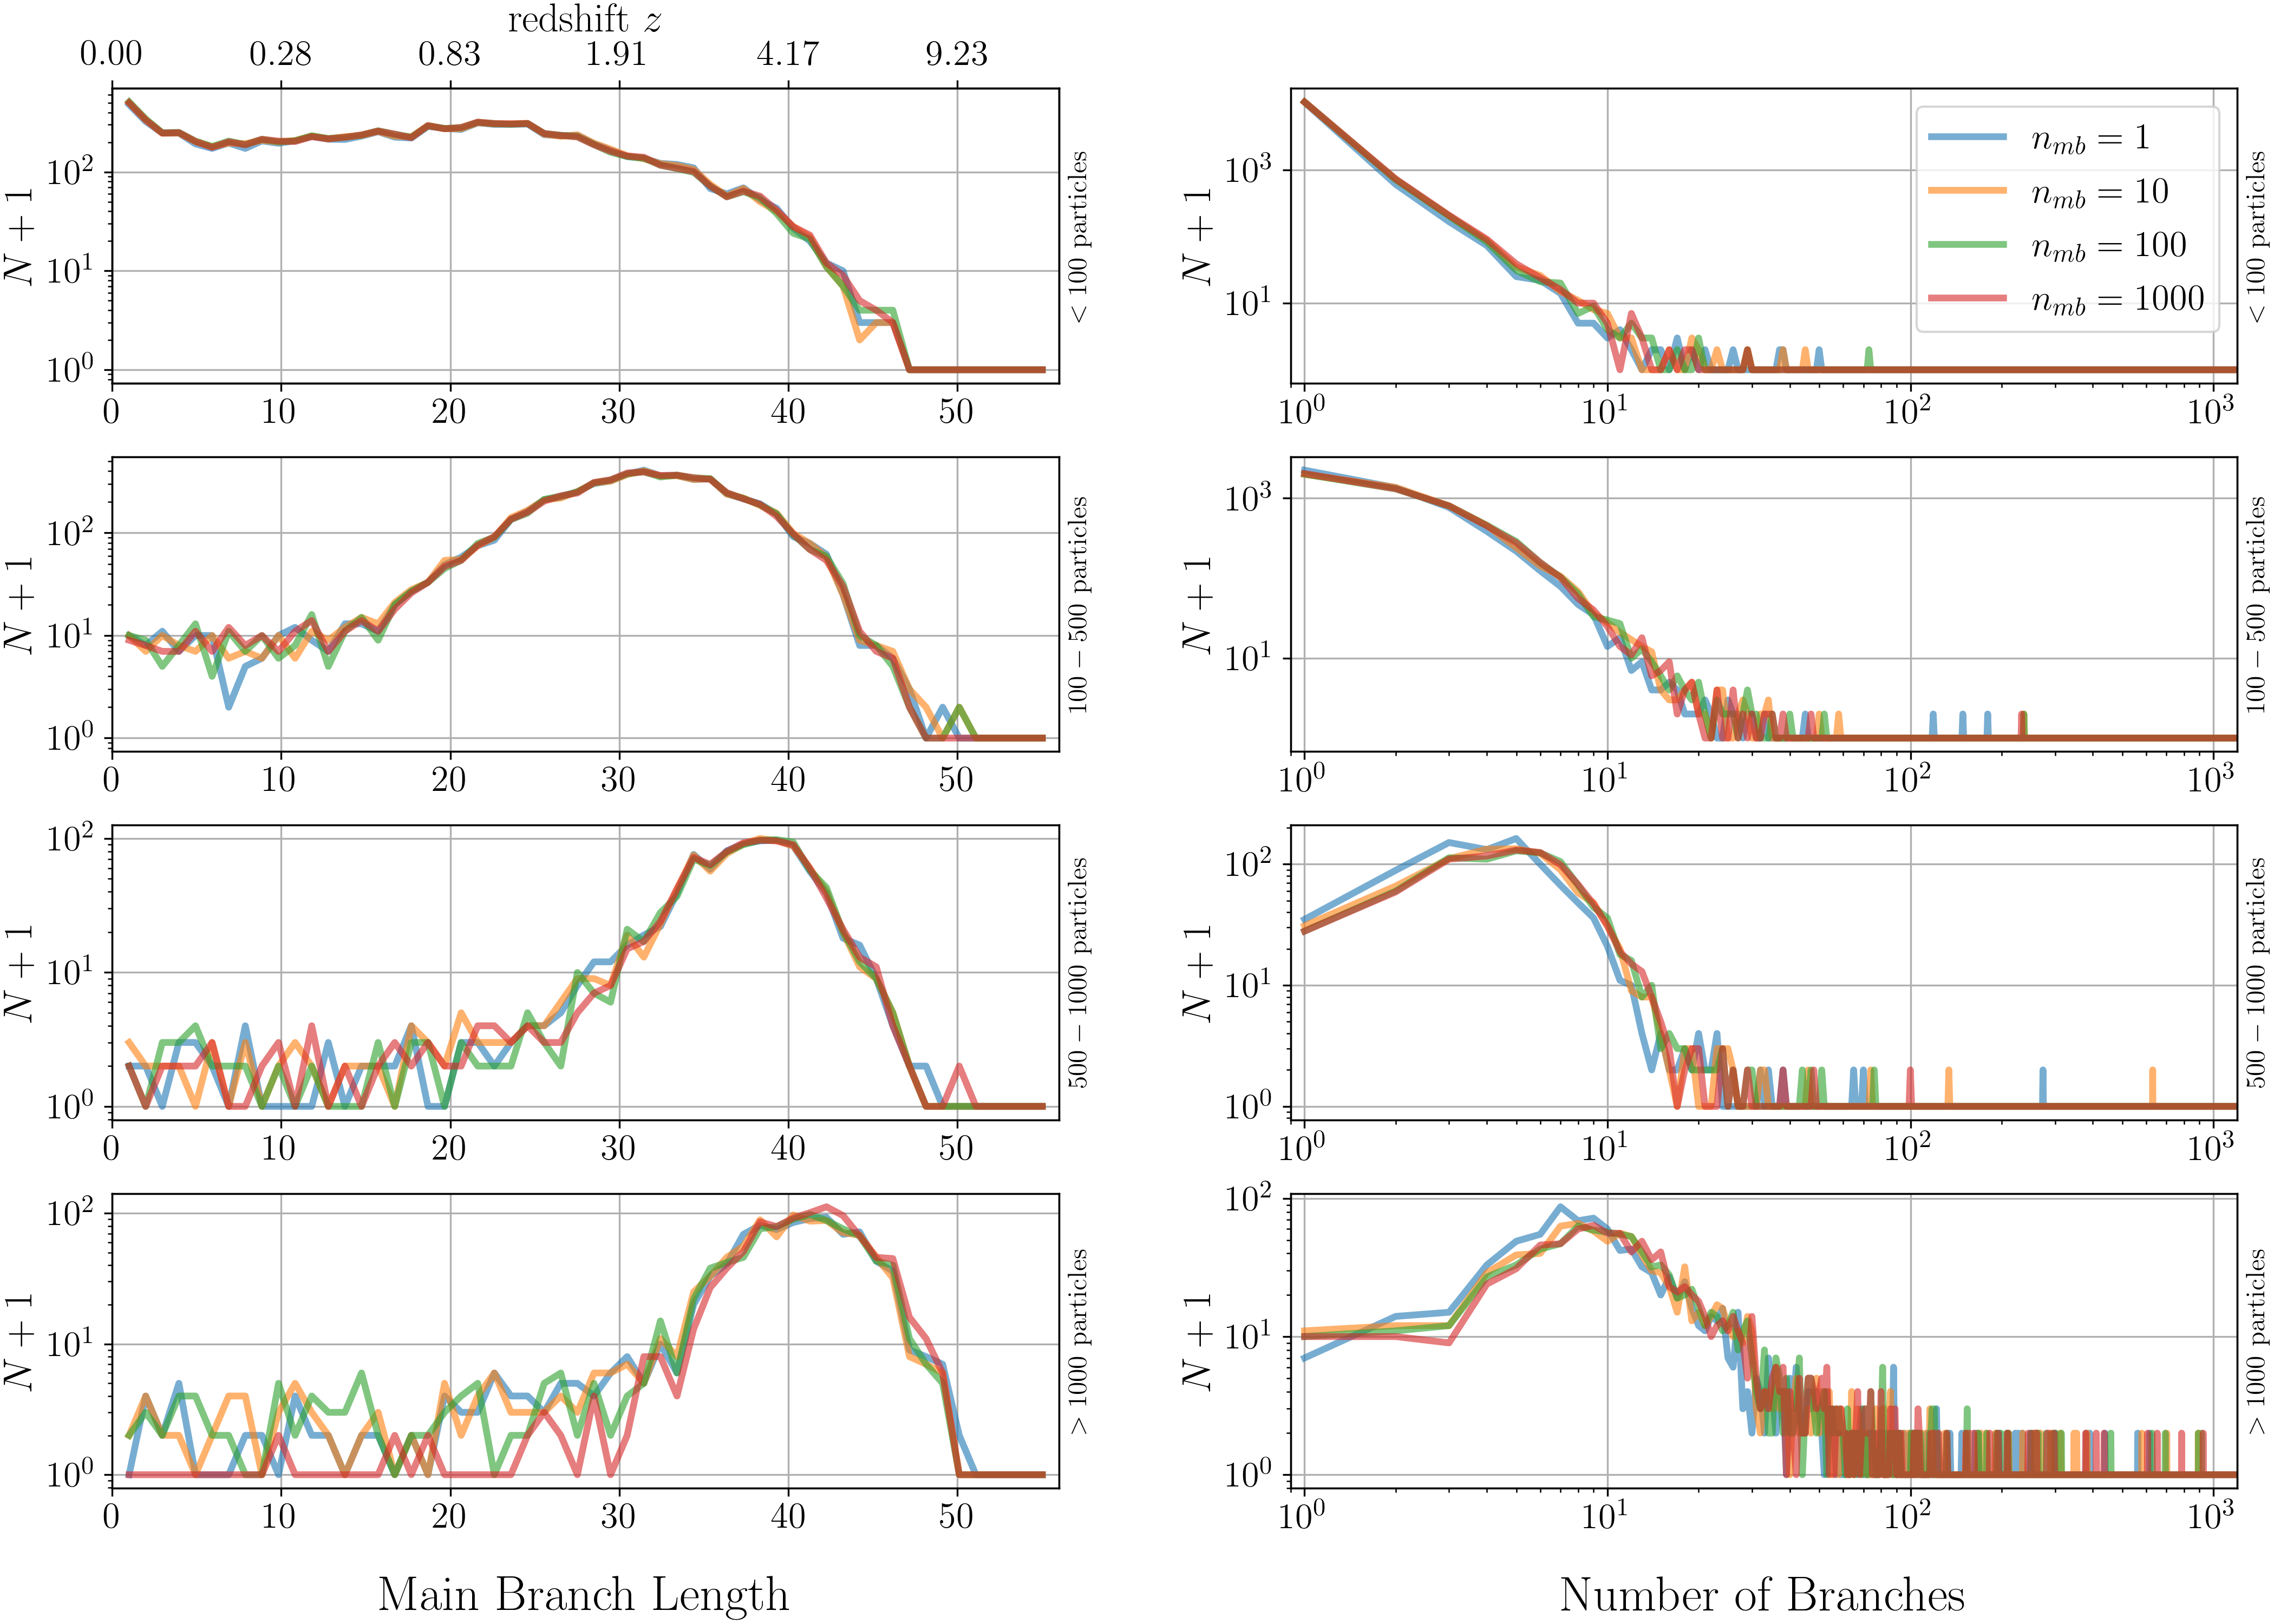
\includegraphics[width=\textwidth, keepaspectratio]{images/tree-statistics-my-threshold/tree_geometry-ntrace.png}%
  \caption{ Histogram of the length of the main branch (left) and
    histogram of the number of branches (right) for all clumps (haloes
    and sub-haloes) detected at $z=0$ for different numbers of tracer
    particles $n_{\rm mb}$ indicated in the legend.  Each row
    corresponds to a different range of clump masses (expressed in
    particle numbers): less then 100 (top), 100-500, 500-1000 and more
    than 1000 (bottom).  In all cases, we used the \exc\ and
    \sad\ clump mass definitions.
  }%
  \label{fig:ntracers_mbl_nbranch}
\end{figure*}

\begin{figure}
  \centering
  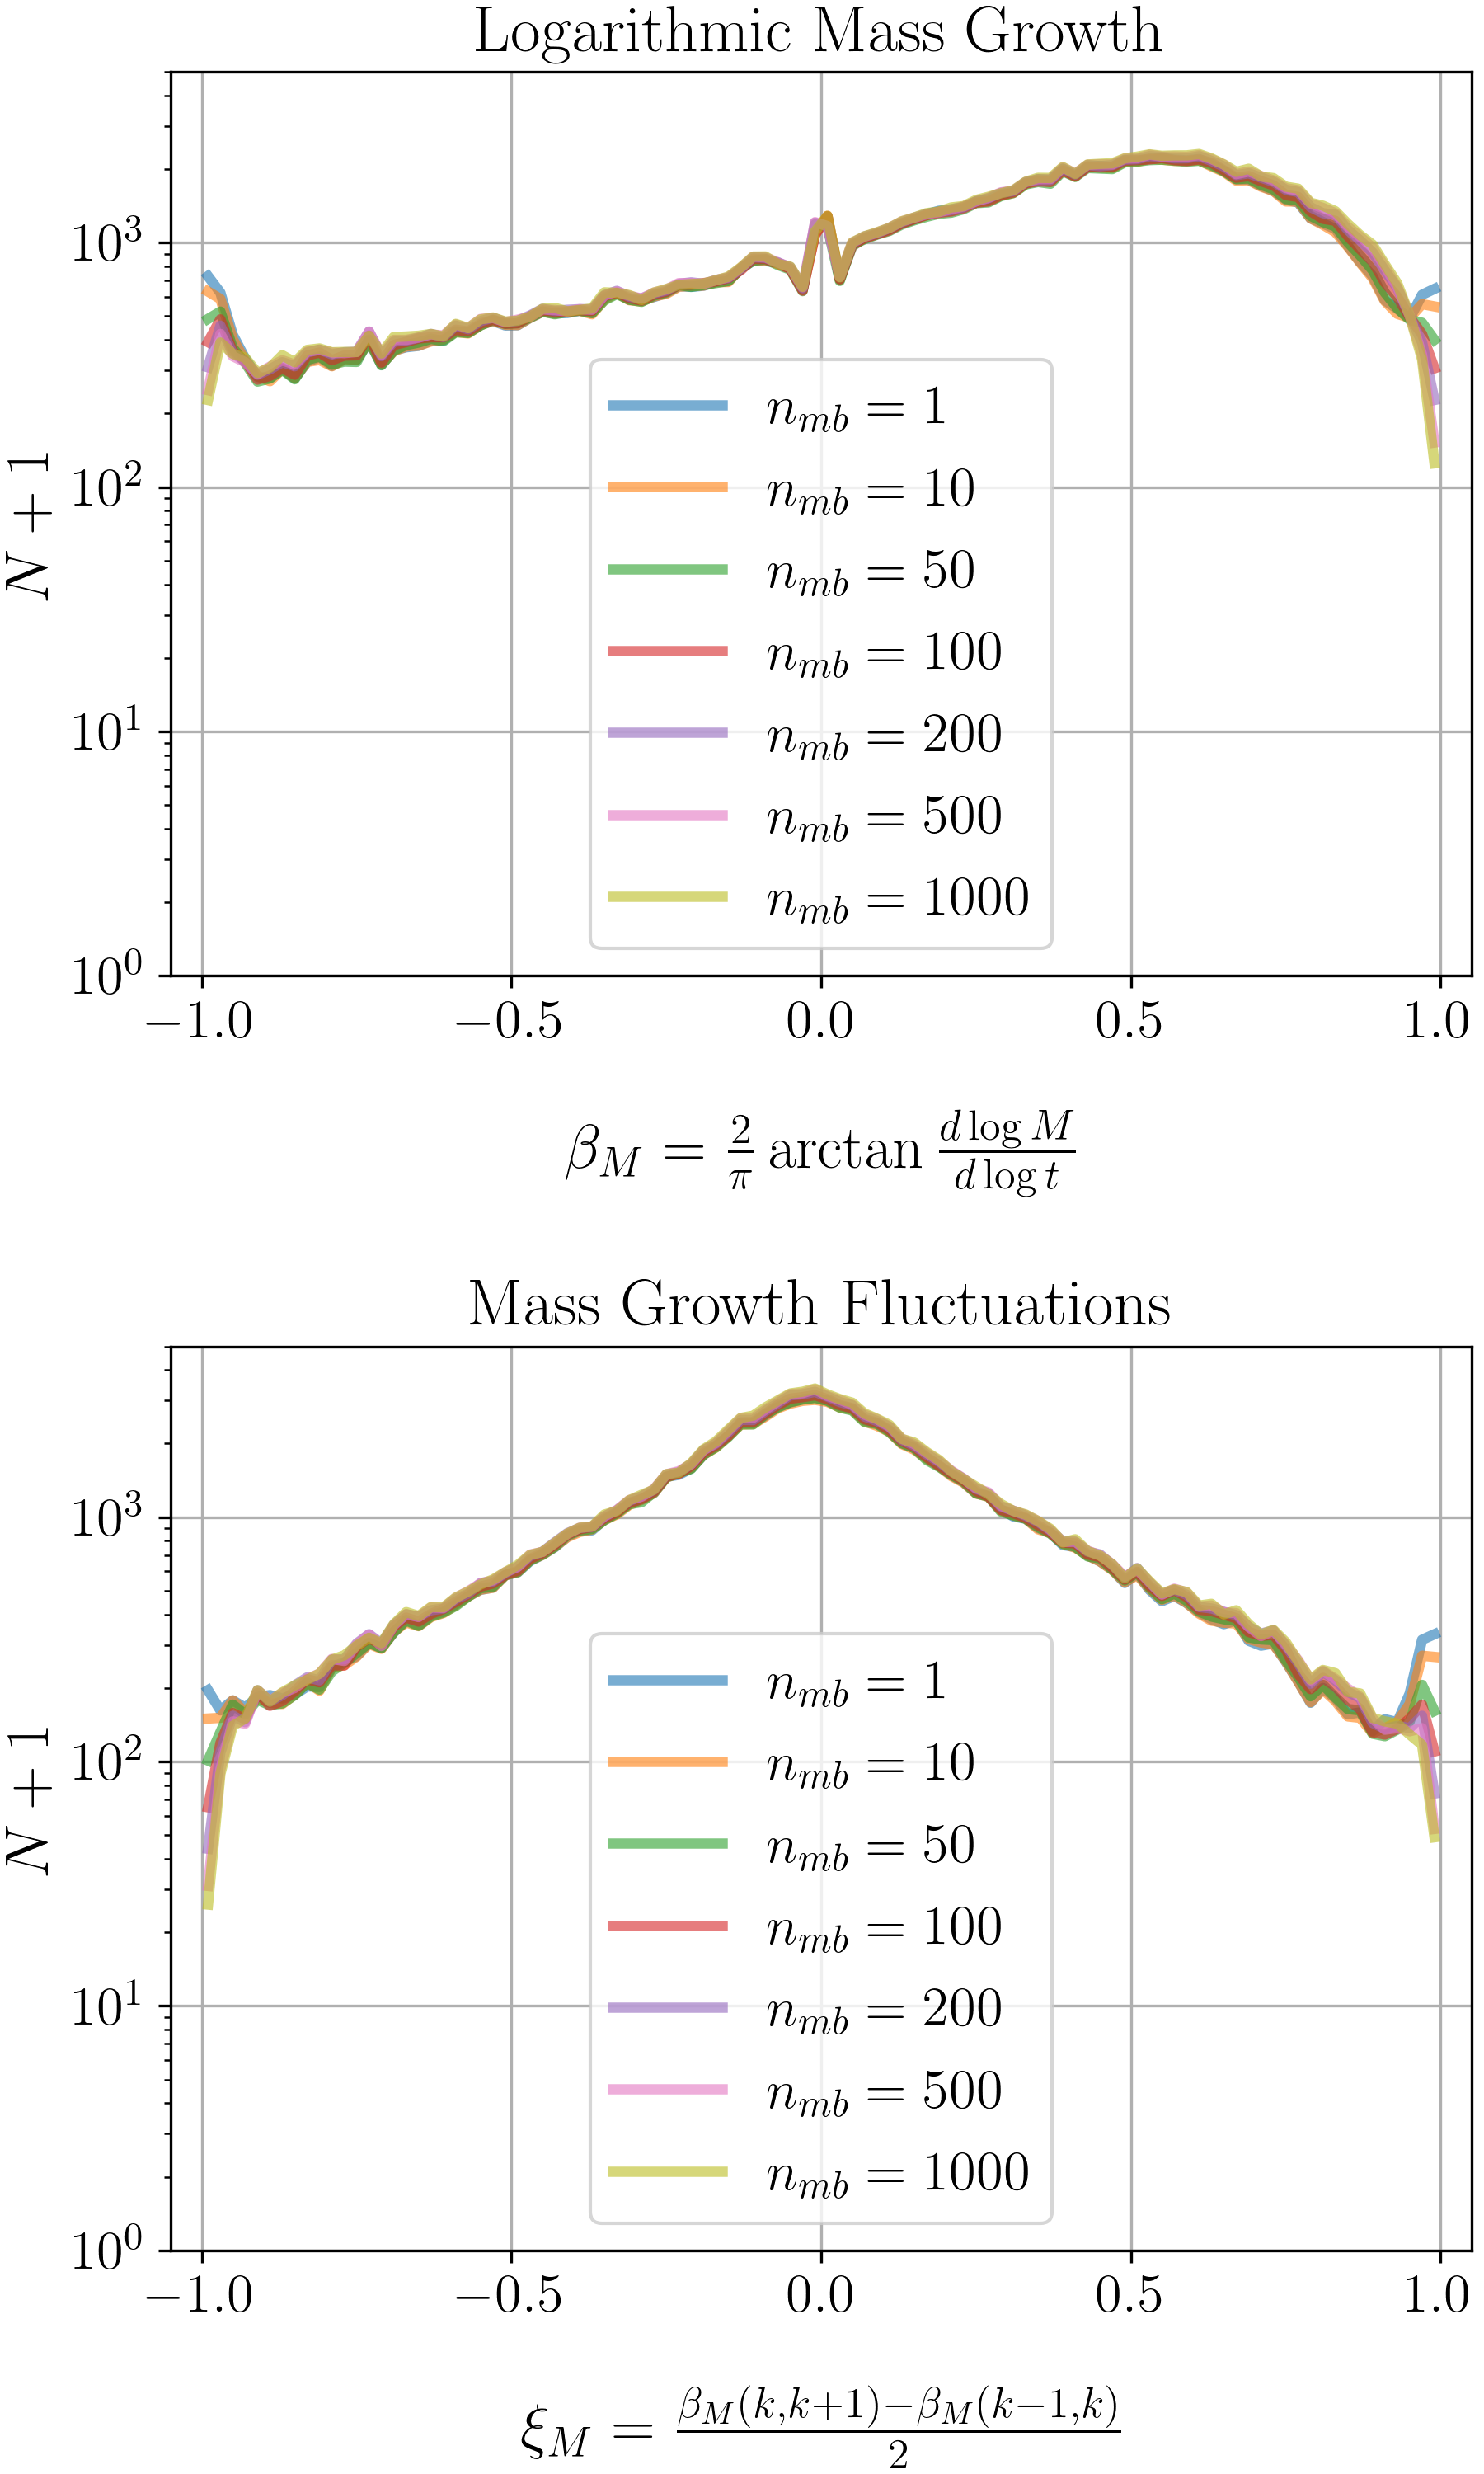
\includegraphics[width=.9\linewidth, keepaspectratio]{images/tree-statistics-my-threshold/mass-statistics-ntrace.png}%
  \caption{ Histogram of the logarithmic mass growth (top) and
    histogram of the mass growth fluctuation (bottom) for all clumps
    (halo and sub-halo) detected in two (top) or three (bottom)
    consecutive snapshots of the simulation and with more than 200
    particles.  We compare these histograms for four different numbers of
    tracer particles $n_{\rm mb}$ as indicated in the legend.  In all
    cases, we used the \exc\ and \sad\ clump mass definitions.
  }%
  \label{fig:ntracers_masses}
\end{figure}

\begin{figure}
  \centering
  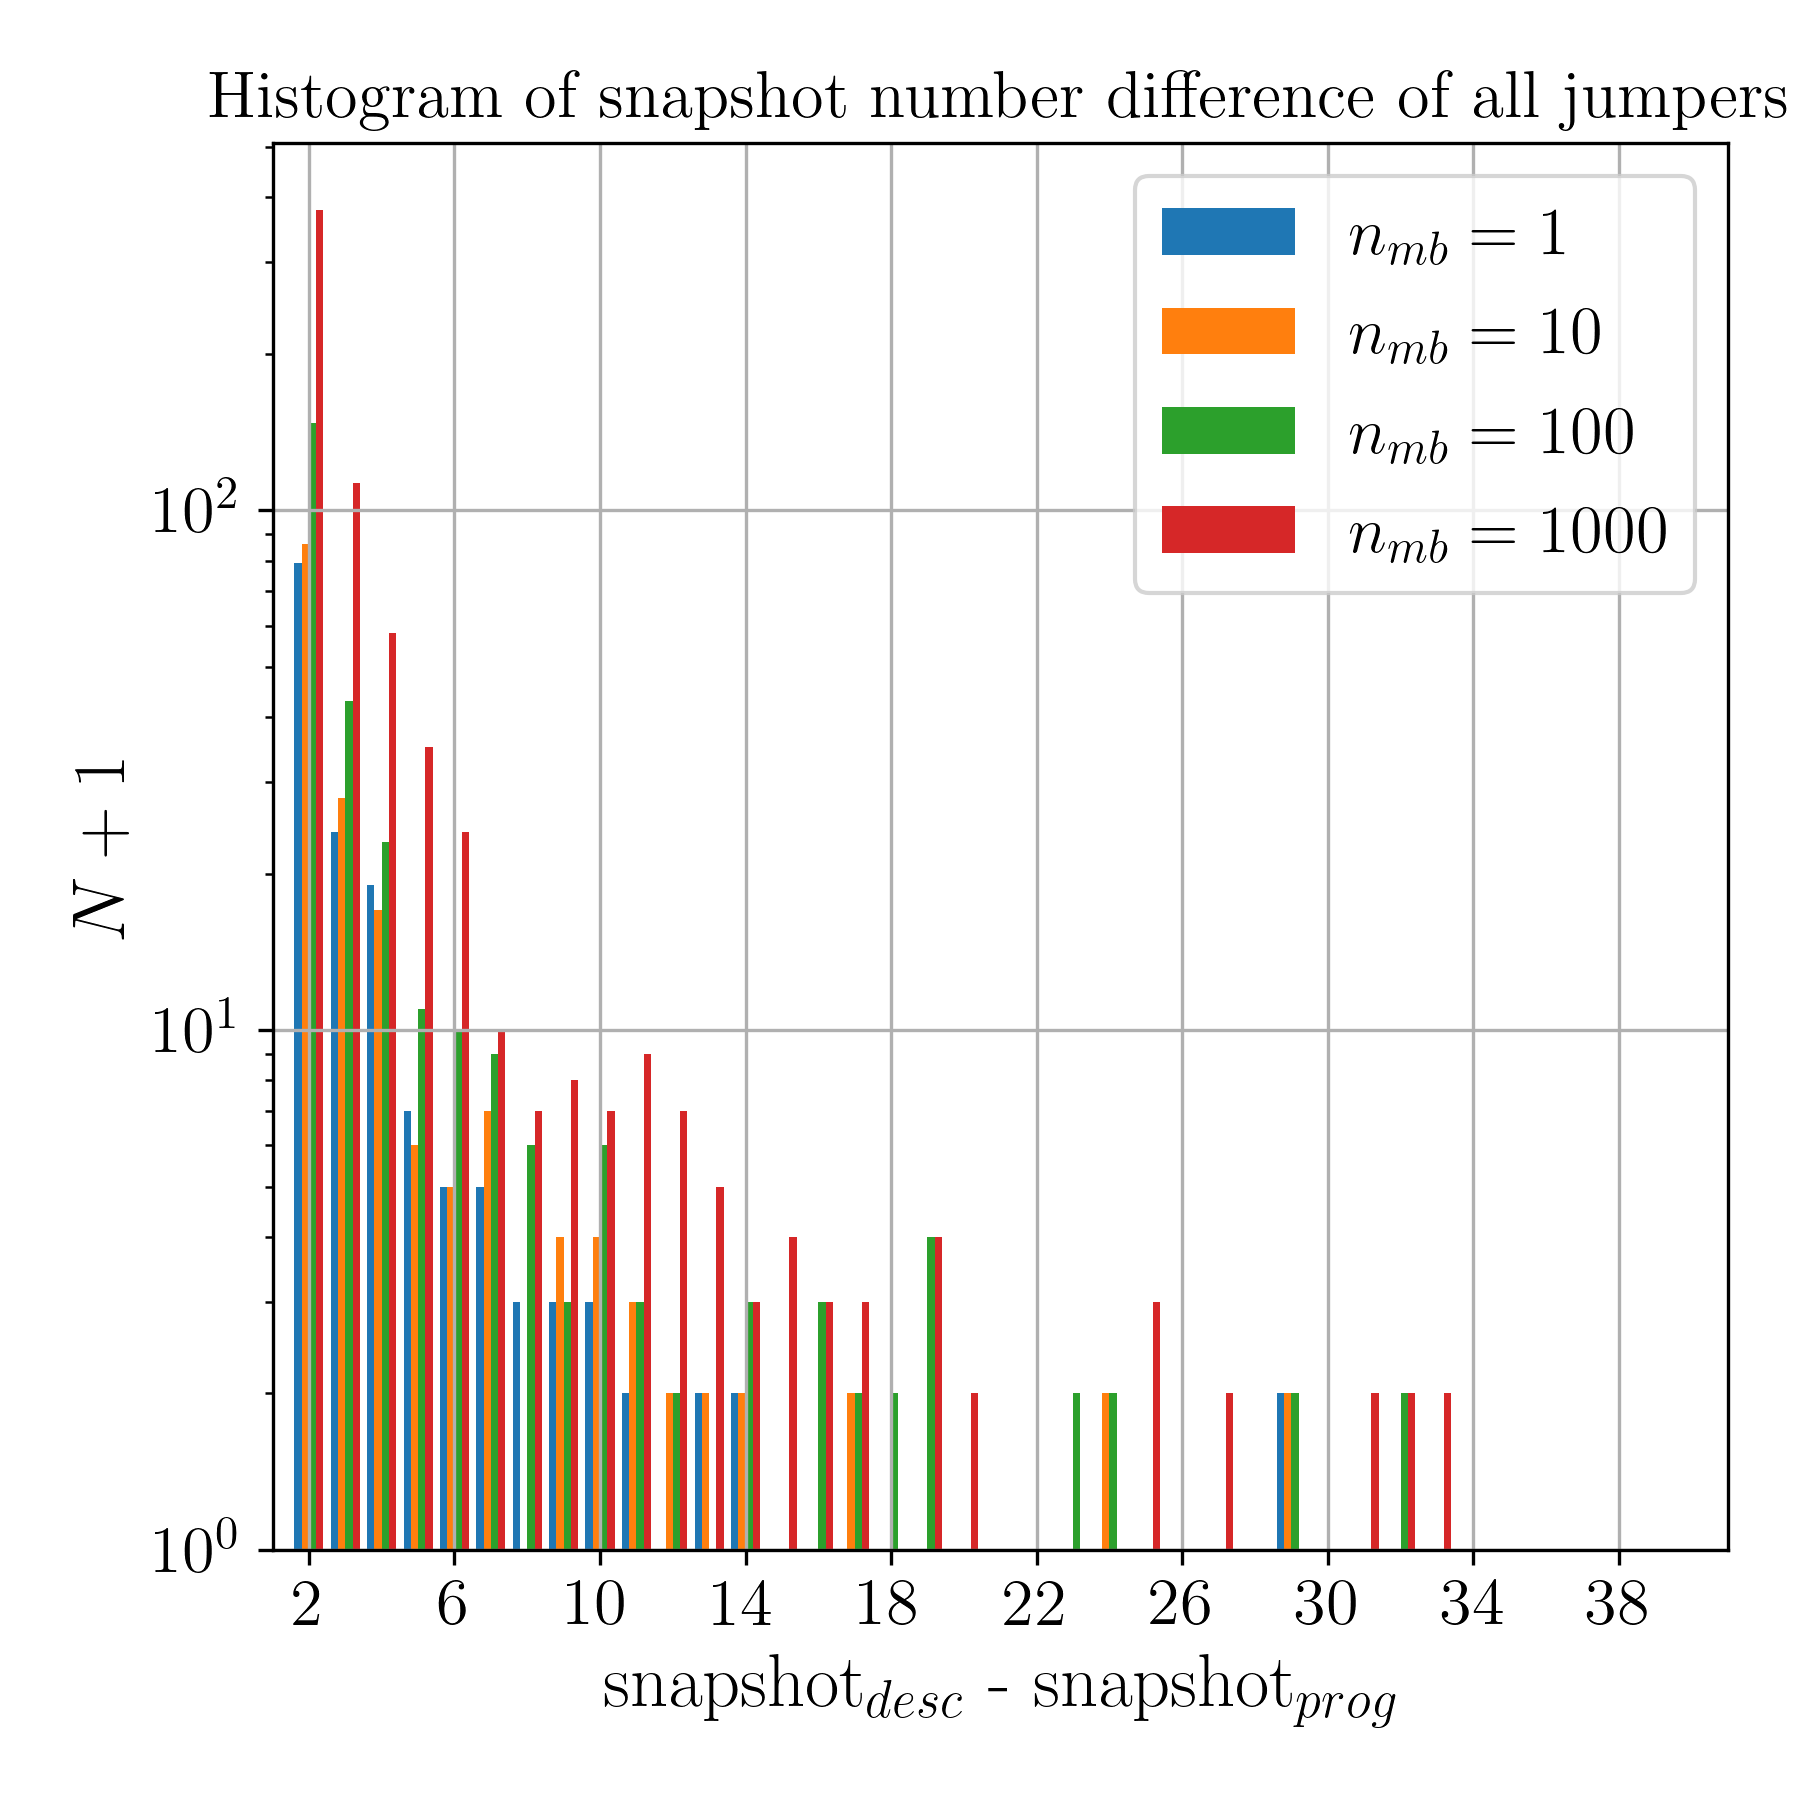
\includegraphics[width=.9\linewidth, keepaspectratio]{images/tree-statistics-my-threshold/jumper_distance-ntrace.png}%
  \caption{ Histogram of the difference in snapshot numbers for
    jumpers, i.e.  progenitor-descendant links which are made across
    non-adjacent snapshots.  Only pairs where both the progenitor's
    and the descendant's masses exceed 200 particle masses were
    included in this plot.  We compare these histograms for four
    different numbers of tracer particles $n_{\rm mb}$ as indicated in
    the legend.  In all cases, we used the \exc\ and \sad\ clump mass
    definitions.
  }%
  \label{fig:jumper-distances}
\end{figure}

\begin{figure}
  \centering
  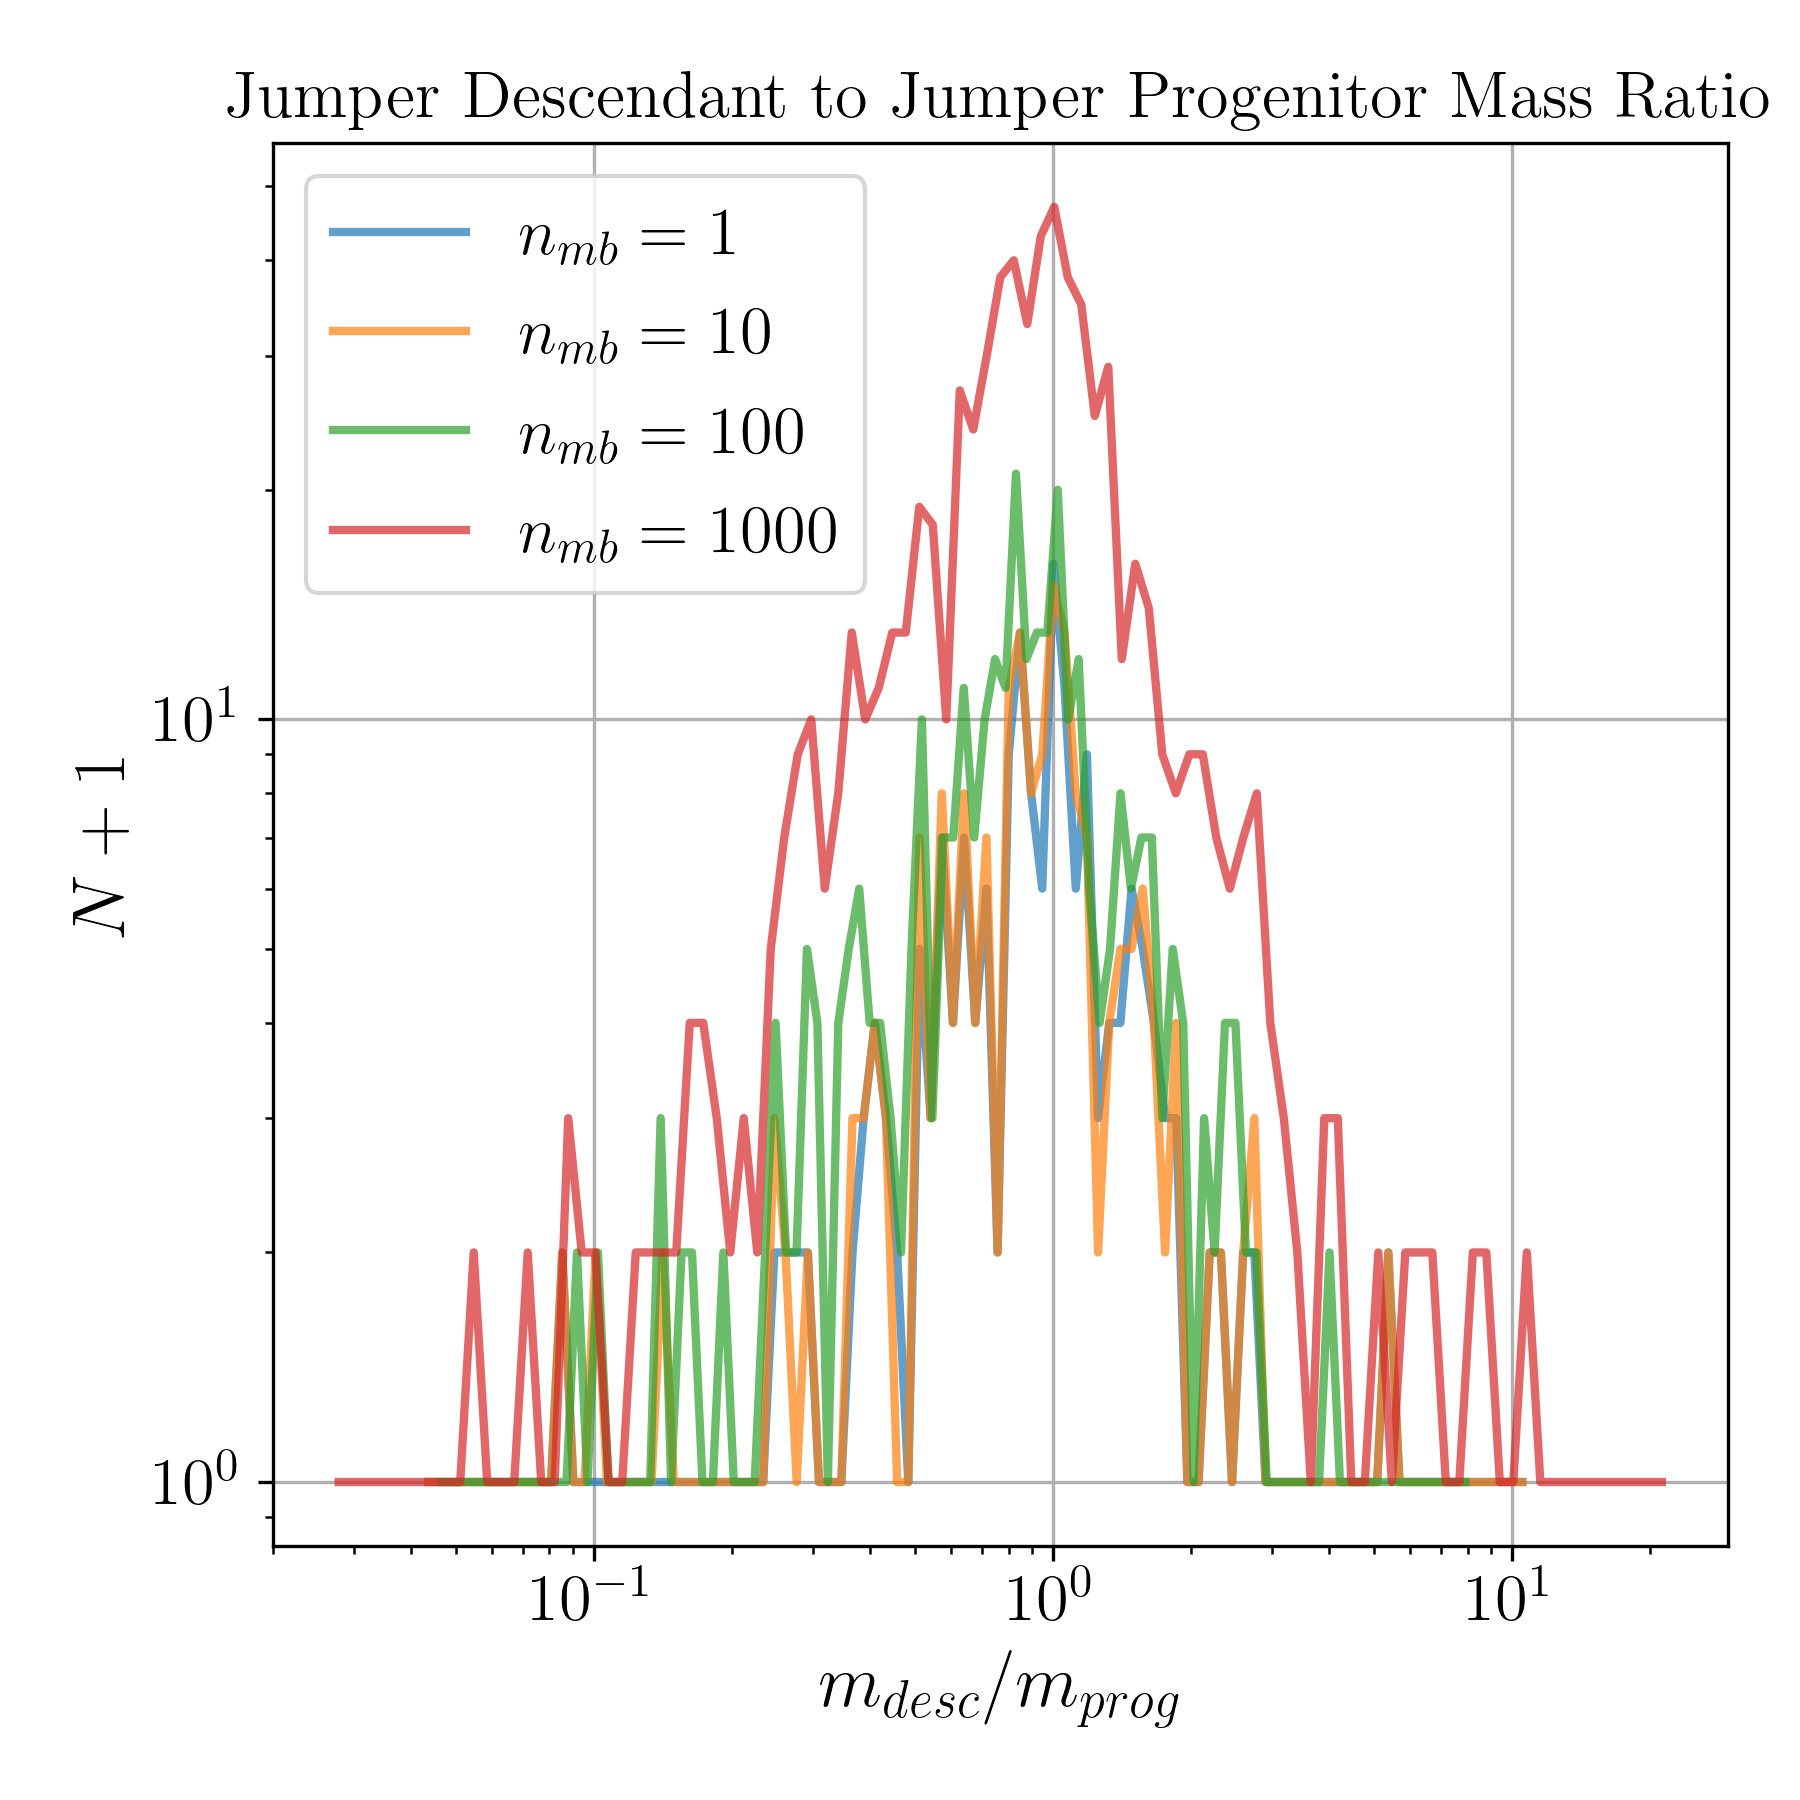
\includegraphics[width=.9\linewidth, keepaspectratio]{images/tree-statistics-my-threshold/jumper_mass_ratio-ntrace.png}%
  \caption{ Histogram of the ratio of descendant mass to progenitor
    mass for jumpers, i.e.  progenitor-descendant links which are made
    across non-adjacent snapshots.  Only pairs where both the
    progenitor's and the descendant's masses exceed 200 particle
    masses were included in this plot.  We compare these histograms
    for four different numbers of tracer particles $n_{\rm mb}$ as
    indicated in the legend.  In all cases, we used the \exc\ and
    \sad\ clump mass definitions.
  }%
  \label{fig:jumper-mass-ratio}
\end{figure}


In this section, we study the effect of varying the number of tracer
particles on our various diagnostics of tree quality. 
Even though we performed the simulations with
up to 1000 tracer particles, the mass threshold for clumps was always
kept constant at 10 particles. The number of tracer particles per clump 
is an upper limit, not a lower limit. For clumps that contain less than 
$n_{\rm mb}$, this means that they will be traced by every single 
particle they consist of. In effect, we expect that this assigns greater
weight to clumps which are more massive than $n_{\rm mb}$ to be identified 
as the main progenitor, and should hopefully decrease extreme 
mass growths and mass fluctuations. To illustrate, consider for example the 
merging of two clumps with unequal masses, where
all of the tracer particles of both clumps are found inside the resulting
merged descendant. Raising the number of tracer particles above the less
massive clump's particle number in this scenario means that the number of
its tracer particles inside the descendant will remain constant, while
the number of tracer particles stemming from the more massive clump will
increase, and thus raising its merit to be the main progenitor. This is 
also the desired outcome. 
Should however both clumps have masses above $n_{\rm mb}$ particle masses,
then our inclusion of the clump masses in the merit function should 
nevertheless find the more massive clump to be the main progenitor if it
had a mass closer to the resulting descendants mass. So we expect that 
increasing the number of tracer particles should enhance this effect,
and hence lead to at least as smooth mass growths and fluctuations.



We show in
Table~\ref{tab:ntracers} the average number of branches and the
average length of the main branch for all our detected clumps at $z=0$
organised in different mass bins. We see that the effect of the number
of tracer particles used is quite mild. Even with as few as one tracer
particle do we manage to recover the correct average main branch
length. This is also true for small mass haloes, although with a
slightly reduced accuracy. This also validates our orphan particle
technique to track temporary merger events.

On a closer look, the average number of branch is however more
affected by the number of tracer particles. If we look at the two highest
mass bins for clumps in the two bottom rows of Table~\ref{tab:ntracers},
we can see that the average number of branches converges towards
the values of 1000 tracer particles used, and is only slightly lower in
the cases when 200 or 500 tracer particles were used. Comparing these
converged results to the ones with only one tracer particle, 
we loose $\sim 30\%$ of the average number of branches, which are 
links associated to merger events.  This
can be easily explained by the fact that too few tracer particles
cannot be distributed across enough descendant candidates to identify
potential links. It appears that using 100 tracer particles is enough 
to recover most of the otherwise broken links. These
conclusions remain the same after looking at the histogram of the
number of branches and the histogram of the main branch length for the
same clumps in Figure~\ref{fig:ntracers_mbl_nbranch}. Here again, we
see the peak of the histogram of the number of branches being shifted
to the right when increasing the number of tracer particles. We also
see that using 100 tracer particles seems enough to almost recover the
correct distribution.

We now examine the effect of the number of tracers on the mass growth
(and on the mass growth fluctuations) of all our detected clumps
within the entire redshift range. We see in
Figure~\ref{fig:ntracers_masses} that the effect is very weak, except
for the extreme cases $\beta_M \simeq \pm 1$ and $\xi_M \simeq \pm 1$,
corresponding to spurious links in the merger tree. These extreme mass 
growth cases correspond to broken links due to the
small number of tracer particles. Here again, using more than 100
tracer particles seem to get rid of most of these spurious cases.
Note that we include in these histograms only clumps with more than
200 particles.

We now study in details another spurious effect of our merger tree
algorithm, shared by many other merger tree code in the literature,
namely dead tree branches.  A dead branch arises when no descendant
could have been identified after a certain redshift, even after
looking for all subsequent snapshots using the corresponding orphan
particle. Such an event is called a ``Last Identifiable Descendant In
Tree'' or LIDIT.  When such a case occurs, it is customary to prune
the corresponding tree from the tree catalogue. When not enough tracer
particles are used, we expect such spurious dead links to
appear. Table~\ref{tab:ntracers-pruning} shows the statistics of these
LIDITs (or tree pruning events), which confirms that the number of
LIDITs decreases strongly when using more and more tracer
particles. We also show in the same table the typical and maximum mass
of the LIDITs. Interestingly, the maximum mass also strongly decreases
when using more tracer particles. When enough tracer particles are
used, we see that LIDITs are typically less massive than 200
particles. We believe they correspond to poorly resolved clumps that
are subject to all sorts of spurious numerical effects. We found that
taking all LIDITs into account, over 80\% of them were main haloes.
LIDITs containing more than 50 particles however were over 95\% sub-haloes.
This suggests that the number of very low mass LIDITs is dominated
by poorly resolved small clumps in low density environments, since
in overdense environments clumps wouldn't have been identified as main 
haloes, but as sub-haloes instead. Conversely, with increased resolution 
of the clumps, the overwhelming majority of LIDITs are sub-haloes, and as
such in overdense regions. We conclude that a
conservative resolution limit of 200 particles per clump removes all the
LIDITs from our catalogue, as long as one uses more than 200 tracer
particles. 

We finally study a specific aspect of our merger tree algorithm,
namely the possibility to follow the temporary mergers of clumps that
travel through another clumps to emerges later as a distinct object.
We show in Table~\ref{tab:jumpers} the number of these temporary
mergers that we call ``jumpers'' as they represent links across
non-adjacent snapshots that we are able to ``repair'' using orphan
particles. On average, the number of jumpers increases with the
number of tracer particles. This is a similar behavior than for the
number of branches: More tracer particles allows more merger events to
be detected, and every merger event results in a new orphan particle.
More orphan particles allow more non-adjacent descendant candidates
to be found. We here also recommend to use 200 tracer particles as a
compromise between speed and proper detection of jumpers in the
simulation.

We show in Figure~\ref{fig:jumper-distances} the histogram of the
distance in time between the two non-adjacent snapshot of all jumpers
in our merger tree. We see that most jumpers have a distance of only 2
snapshots. They corresponds to clumps traversing another clump and
re-emerging a snapshot later as a distinct halo. We also see in
this histogram that the number of jumpers increases with the number of
tracer particles. But overall, the statistics of the distance between
jumpers is relatively robust, with only very rare cases with a
distance larger than 10 snapshots. Figure~\ref{fig:jumper-mass-ratio}
shows the histogram of the mass ratio between the jumper progenitor
and the jumper descendant.  As expected, it peaks at one, which means
that the mass of the clump that re-emerges in a later snapshot is
close to the mass of the clump that disappeared in an earlier
snapshot. Note that this is not due to the merit function, because for
jumpers we only use a single orphan particle to repair the link. This
is a clear sign that the same clump is identified before and after the
temporary merger.  We also see that the distribution is slightly
skewed toward mass ratio smaller than 1, with values always bounded
between 0.3 and 3. Only a few very rare cases show more extreme mass
ratios. This means that clumps hosting our orphan particles either
preserve their mass (over 2 snapshots) or loose mass (on average),
usually when the time between non-adjacent snapshots increases.

In conclusion, we found that $n_{\rm mb} \simeq 200$ is a safe choice
to obtain robust results for our merger tree algorithm, in light of
the diagnostics we have used in this section.  We also recommend
adopting a conservative mass threshold of 200 particles per clumps to
get rid of a few rare spurious dead branches that would need to be
pruned from the halo catalogue anyway.
